\documentclass[twocolumn,amsmath,amssymb,pra, floatfix]{revtex4-2}
\usepackage[utf8]{inputenc}
\usepackage{graphicx}
\graphicspath{ {figures/} }
\usepackage{siunitx}
\usepackage{hyperref}
\usepackage{float}

\begin{document}

\title{Physics 360-0: Rubidium Spectroscopy}

\author{Jun Sung, Maura Lally}

\date{05-18-21}

\begin{abstract}
The purpose of this lab is to observe and measure the hyperfine splitting of a rubidium vapor cell. To achieve this purpose, we utilized the TeachSpin diode laser and controller to perform a saturated absorption spectroscopy. Doing so allowed for us to unveil the hyperfine structure of the rubidium vapor cell, and the controller further allowed for us to "zoom" in on the hyperfine structure for each of the resonant peaks (four in total in our case). We note that we displayed the output of the controller using an oscilloscope, where we further note that the default horizontal scale is in terms of time. However, in order to actually measure the peaks (or the difference in frequency between them, that is), we need to incorporate an interferometer so that we can associate the time intervals displayed on the oscilloscope with frequency intervals. With this in place, we are able to measure the hyperfine splitting from the oscilloscope. The expected values and results that we got can be found Table \ref{tab:results}, and we find that most of our results are within $1 \sigma$ of the expected values. 
\end{abstract}

\maketitle

\section{Introduction}
In 1913, Niels Bohr used the relatively new theory of quantum mechanics as an explanation for the spectral lines of a hydrogen atom \cite{wiki:QMhist}. Over the following years/decades, quantum mechanics solidified itself as a fundamental theory that provides a thorough understanding and description of the physical properties of nature at the scale of atoms and subatomic particles \cite{wiki:QM}. It is quantum mechanics that led to our understanding of semiconductors, which further led to the diode lasers that we make use of in this lab. In a way, quantum mechanics comes full circle with this lab; we will be studying the hydrogen-like rubidium atom and will try to verify what we expect from quantum mechanics. 

\subsection{Brief Overview of Methods}
Most generally, our goal is to understand how the properties of rubidium can interact with light, and how light might be used to probe the properties of rubidium. In particular, our main focus will be on the hyperfine splitting of rubidium. To achieve this goal, we will run three experiments: the first will be on observing the absorption spectrum for a rubidium vapor cell; the second will be on observing the p-state hyperfine splitting for a particular peak in the absorption spectrum; and finally, the third will be to measure the hyperfine splitting for each of the peaks in the absorption spectrum, collect results, and compare those results with what we expect to find from theory.

\subsection{Applications} 
The methods that we apply in this lab, namely that of spectroscopy, can be applied more broadly to many areas of study. Environmental scientists in particular use many types of spectroscopy in their studies \cite{spectroscopy_applications}. For example, emission spectroscopy can be used to determine what elements are present in a given sample of water or solids.

Spectroscopy also finds uses in astronomy, and it can tell us about the composition, density, and temperature of certain astronomical objects \cite{spectroscopy_applications}. Astronomers are also able to use spectroscopy to measure the red-shifting of light that comes from stars and galaxies. This measurement further allows for us to calculate the relative velocities of such stars and galaxies.

A few more applications of where spectroscopy can be used would be: determining the metabolic structure of a muscle, altering the structure of drugs to improve effectiveness, and characterizations of proteins \cite{pasco}.

\section{Theory} 
One of the conclusions that quantum mechanics was able to provide when trying to explain the spectral lines of a hydrogen atom was that an electron bound to the hydrogen atom could only take on discrete values of energy. The discretization of energy didn't only hold to this case; it was found to be a general phenomenon for atoms in general. However, as more was known about the behavior of these atoms/particles, it was found that the spectra of atoms split into more than just energy levels -- these splittings being the fine and hyperfine-structure.

\subsection{The Fine-Structure Splitting of Atomic Spectra}
Although we do not measure the fine-structure splitting of rubidium, it is still important to understand the theory behind this. The fine-structure of an atom refers to the splitting of its spectral lines due to electron spin and relativistic corrections to the non-relativistic Schr\"{o}edinger equation \cite{wiki:FineStructure}. In particular, there are three main corrections that we will discuss: spin-orbit energy corrections, relativistic corrections, and the corrections given by the Darwin shift.

\subsubsection{Spin-Orbit Energy Corrections}
This correction accounts for the energy shift that occurs due to the electromagnetic interaction between the electron's magnetic dipole, its orbital motion, and the electrostatic field of the positively charged nucleus \cite{wiki:SpinOrbitInteraction}. To determine how much of an energy change that we will have, we first note that the magnetic moment of the spinning electron in a magnetic field has potential energy due to its torque given by 
\begin{equation}
    U = - \mu \cdot \mathbf{B}
    \label{eq:soe-1}
\end{equation}
Furthermore, since we know that the electron is orbiting our rubidium atom, the electron generates a magnetic field:
\begin{equation}
    \mathbf{B}
    =
    \frac{ e \mu_{0} }{ 4 \pi m_{e} } \frac{ \mathbf{L} }{ r^{3} }
    \label{eq:soe-2}
\end{equation}
Before we substitute equation \ref{eq:soe-2} into equation \ref{eq:soe-1}, we make note that the electron's intrinsic spin and magnetic moment are related by 
\begin{equation}
    \mu = g_{s} \frac{- e}{2 m_{e}} \mathbf{S}
    \label{eq:soe-3}
\end{equation}
Hence, we see that equation \ref{eq:soe-1} can be rewritten to be 
\begin{equation}
    U 
    = 
    - g \frac{-e}{2 m_{e}} \frac{e \mu_{0}}{4 \pi m_{e} r^{3}} \mathbf{L} \cdot \mathbf{S}
    =
    \frac{g e^{2}}{8 \pi \epsilon_{0} m_{e}^{2} c^{2}} \frac{1}{r^{3}} \mathbf{L} \cdot \mathbf{S}
    \label{eq:soe-4}
\end{equation}
where we have used the fact that $c^{2} = \frac{1}{\epsilon_{0} \mu_{0}}$. We also make note that we will only be studying $p$-states whose orbital angular momentum and intrinsic spin are in the states $l = 1$ and $s = \frac{1}{2}$, respectively. This means that the total angular momentum state is given by $j = \frac{3}{2}$.

Knowing this, we can determine the spin-orbit contributions to the total Hamiltonian, say $H_{S-O}$, by noting that $H_{S-O} = U$. Furthermore, we can determine the energy shift from this spin-orbit contribution by calculating the expectation value of $H_{S-O}$ (the details of the calculation can be found in the lab manual). The result of the calculation gives us the following energy shift via spin-orbits:
\begin{equation}
    \Delta E_{S-O} = \pm g E_{n} \frac{(Z \alpha)^{2}}{6 n} 
    \label{eq:soe-5}
\end{equation}
where 
\begin{equation}
    E_{n} = - \frac{Z e^{2}}{8 \pi \epsilon_{0} a_{0}},
    a_{0} = \frac{4 \pi \epsilon_{0} \hbar^{2}}{m_{e} e^{2}},
    \alpha = \frac{e^{2}}{4 \pi \epsilon_{0} \hbar c}
    \notag
\end{equation}
We note that $E_{n}$ refers to the Bohr energy levels, $a_{0}$ is the first hydrogen radius, and $\alpha$ is the fine-structure constant. As for the $\pm$ that occurs in equation \ref{eq:soe-5}, they occur when the electron has "spin down" or "spin up" in the $p$-state, respectively. In fact, the fine-structure lines are separated by the difference or twice the absolute value. We should further note that the $s$-states have no angular momentum, no orbital current, and thus no spin-orbit interaction

\subsubsection{Relativistic Corrections}
The electron's kinetic energy is more correctly given by 
\begin{align}
    T
    &= 
    \sqrt{(p c)^{2} + (m_{e} c^{2})^{2}} - m_{e} c^{2} 
    \notag 
    \\
    &=
    m_{e} c^{2} \sqrt{1 + \left( \frac{pc}{m_{e} c^{2}} \right)^{2}} - m_{e} c^{2}
    \notag 
    \\
    &\approx 
    m_{e} c^{2} 
    \left(
        1 + \frac{1}{2} \left( \frac{p c}{m_{e} c^{2}} \right)^{2}
        - \frac{1}{8} \left( \frac{p c}{m_{e} c^{2}} \right)^{4}
    \right) 
    - m_{e} c^{2} 
    \notag
    \\
    &=
    \frac{p^{2}}{2 m_{e}} - \frac{p^{4}}{8 m_{e}^{3} c^{2}}
    \label{eq:rc-1}
\end{align}
Notice that the first term is the classical kinetic energy that is already incorporated into Schr\"{o}dinger's equation. As for the second, we need to use perturbation theory to calculate the resulting energy shift. The details can again be found in the lab manual, and we find such an energy shift to be 
\begin{equation}
    \Delta E_{\mathrm{ref}}
    =
    - Z E_{n} \frac{\alpha^{2}}{n^{2}} 
    \left(\frac{3}{4} - \frac{2 n}{3} \right)
    \label{eq:rc-2}
\end{equation}
where we again note that we take the orbital angular momentum state to be $l = 1$.

\subsubsection{Darwin Shift Corrections}
The last of the corrections comes from the Darwin shift. Since we are not measuring the fine-structure splitting of rubidium and are just including this correction for completeness, it suffices to just make note of the energy shift caused by the Darwin shift (the details can again be found in the lab manual):
\begin{equation}
    \Delta E_{\mathrm{Darwin}}
    =
    - Z E_{n} \frac{\alpha^{2}}{n}
\end{equation}

With all the corrections mentioned, we note that the spin-orbit interaction is the only one that splits the energy degeneracy. However, to fully understand and explain the actual energy differences between 5$s$ and 5$p$ fine-structure lines, we need to include the effects from special relativity and the Darwin effect.

\subsection{The Hyperfine Splitting of Atomic spectra}
The hyperfine-structure arises through two main contributions: the magnetic dipole-dipole interaction and the electric quadrupole-quadrupole interaction. Both of these contributions provide an energy shift that further results in the hyperfine splitting of atomic spectra. Because the exact details for how one might obtain the energy shifts are quite technical (Please confer with \cite{gatech} for such technicalities), we will just provide the corresponding energy shifts for both contributions as we did with the fine-structure section of this lab report. 

As stated in the lab manual, the energy shift from the magnetic dipole-dipole interaction is given by
\begin{align}
    \Delta E_{M1}
    &=
    - \mu_{N} \cdot \mathbf{B}_{e}
    \notag 
    \\
    &=
    \pm 
    \left( \frac{g_{n} \mu_{N}}{\hbar} \right) 
    \left( \frac{\mu_{B}}{\hbar} \right) 
    \left( g \mathbf{I} \cdot \mathbf{L} + g_{s} \mathbf{I} \cdot \mathbf{S} \right)
    \label{eq:hfs-1}
\end{align} 
where $\mu_{N}$ is the magnetic dipole moment of the nucleus and $\mathbf{B}_{e}$ is the magnetic flux density due to the atomic electron. It should also be made clear that $g_{N}$ is the gyromagnetic ratio of the nucleus, $\mu_{B}$ is the Bohr magneton, and $\mathbf{L}$ is the angular momentum of the electron. Furthermore, $\mathbf{I}$ and $\mathbf{S}$ are the intrinsic spin for the nucleus and electron, respectively.

As for the electric quadrupole-quadrupole interaction, we get the energy shift to be (from \cite{gatech})
\begin{equation}
    \Delta E_{E2} 
    =
    \alpha
    \left[ 
        \frac{3}{4} C^{2} - \frac{3}{4} C - I (I + 1) J (J + 1)
    \right]
    \label{eq:hfs-2}
\end{equation}
where 
\begin{equation*}
    \begin{gathered}
        \alpha \frac{\beta}{2 I (2 I - 1) J (2 J - 1)} 
        \\[2mm]
         C = F (F + 1) - I (I + 1) - J (J + 1)
    \end{gathered}
\end{equation*}
and $\beta$ is some constant of proportionality with dimensions of energy. 

\subsection{Atomic Structure of Rubidium}
\label{sec:structure}
As stated in the lab manual, the ground-state electronic configuration of rubidium consists of closed shells plus a single 5$s$ valence electron. This configuration is similar to that of a hydrogen atom, and so is the spectrum that we get for rubidium. Rubidium has two naturally occurring isotopes: ${}^{85}\mathrm{Rb}$ (72\% abundance with nuclear spin quantum number $I = \frac{5}{2}$) and ${}^{87} \mathrm{Rb}$ (28 \% abundance with nuclear spin quantum number $I = \frac{3}{2}$). 

\begin{figure}[H]
    \centering
    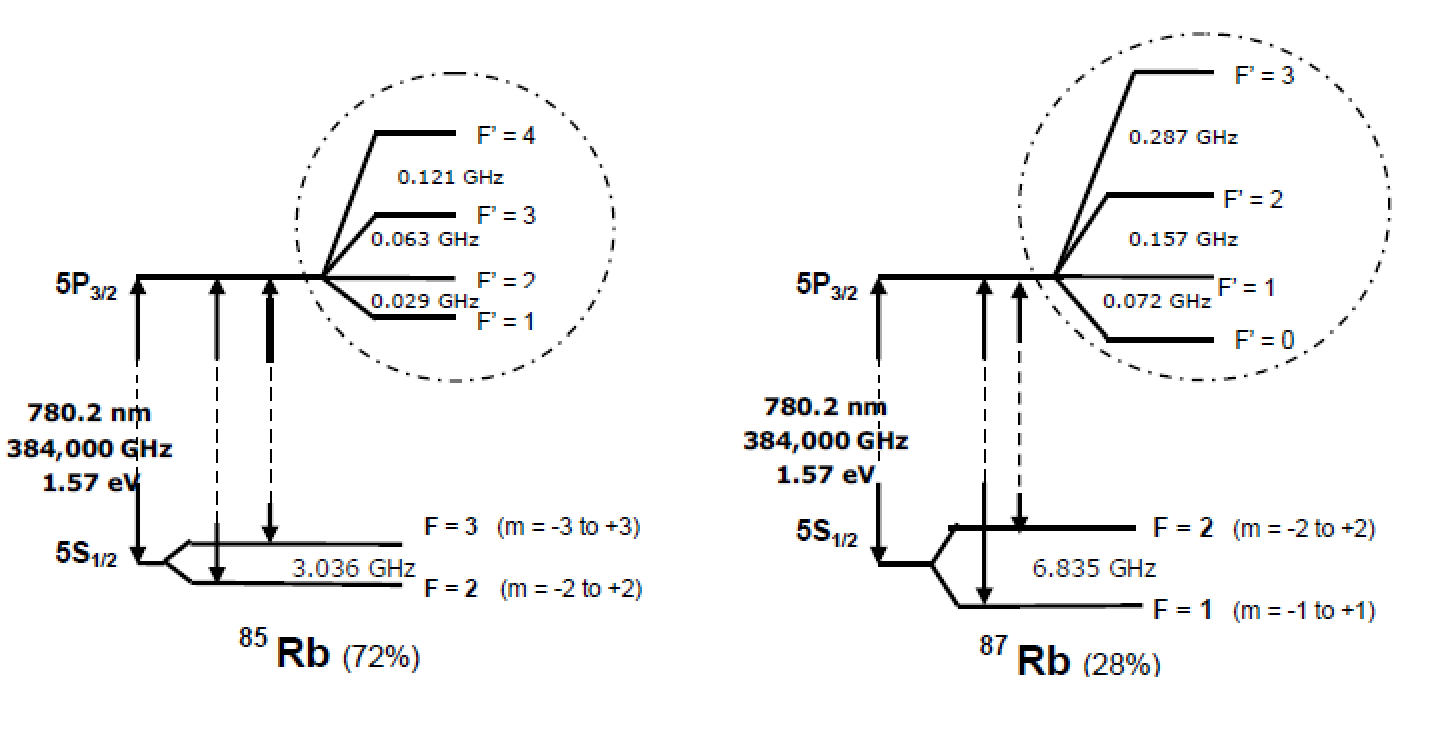
\includegraphics[ width = 0.8 \linewidth ]{Rubidium_Splitting.PNG}
    \caption{Fine and hyperfine splitting of the ground and excited states of rubidium}
    \label{fig:rubidium_splitting}
\end{figure}

Furthermore, both of our isotopes for rubidium have a fine-structure that splits into either $F = 1, 2$ (for ${}^{87}\mathrm{Rb}$) or $F = 2, 3$ (for ${}^{85}\mathrm{Rb}$), and we will denote this splitting as being a or b for both isotopes. For example, if we consider ${}^{85}\mathrm{Rb}$ that splits finely into $F = 2$, then we shall denote this as 85a. 

For either of these isotopes, the first excited state corresponds to when the 5$s$ electron moves up to 5$p$. Because of our laser capabilities, we will only study the $\mathrm{D}_{2}$ line at $780 \si{nm}$ as shown in Figure \ref{fig:rubidium_splitting}. What this corresponds to in our case is that the rubidium isotopes that correspond to $F = 1$ or $F = 2$ will further correspond to the hyperfine splitting of $F' = 0, 1, 2$ or $F' = 1, 2, 3$, respectively. The same can be said for when $F = 2$ or $F = 3$, which correspond to the hyperfine splitting of $F' = 1, 2, 3$ and $F' = 2, 3, 4$, respectively.

\subsection{Doppler Broadening}
The absorption cell consists of an outer glass cylinder, an insulation layer, a heater assembly, a "cold finger", a thermocouple to monitor the temperature, and the gas filled rubidium cell itself. Our main focus will be on the gas filled rubidium cell, and we note that all the gas particles undergo random thermal motion. This random thermal motion ends up resulting in a wider range of frequencies that will be absorbed (other than the frequency of the laser), and this effect is known as Doppler broadening. To explain this effect a little more, let's focus our attention to a single gas particle in our rubidium cell. Furthermore, let's say that our laser is propagating along the $z$-axis, and the velocity of our gas particle has a non-zero component in the $z$-direction. As noted in page 5 of \cite{gatech}, the frequency of the radiation by our gas particle is given by 
\begin{equation}
    \nu_{L}
    =
    \nu_{0} 
    \left( 1 + \frac{v_{z}}{c} \right)
    \label{eq:db-1}
\end{equation}
where $\nu_{0}$ is the resonant absorption frequency for our gas particle at rest, and $v_{z}$ is the $z$-component of our gas particle's velocity. It follows from equation \ref{eq:db-1} that depending on how our gas particle is moving (e.g. towards the laser or away from the laser), the frequency that our gas particle can absorb varies. Hence, because the gas inside of our rubidium undergoes random thermal motion, the range of possible frequencies that our gas can absorb widens due to equation \ref{eq:db-1}. The full details on this effect can be found on pages 5-6 of \cite{gatech}.

The reason why we mention such an effect is because this effect tends to mask more subtle features of our absorption spectra, such as the hyperfine-structure. This is a problem for us since our main goal for this lab is to study the hyperfine-structure of rubidium. However, we can overcome this effect via a saturated absorption spectroscopy. 

\subsection{Saturated Absorption Spectroscopy}
Saturated absorption spectroscopy uses two counter propagating beams at the same frequency with the same group of atoms. This can be seen in the configuration of our apparatus in Figure \ref{fig:apparatus} where the laser splits three beams via BS2, and two beams go through the rubidium vapor cell and land on detectors D1 and D2. The main interest we have with this configuration is that it produces an absorption signal that contains the features that would otherwise be masked by Doppler broadening. The full details on this configuration can be found on pages 6-7 of \cite{gatech}. However, we will make note of one particular feature that arises from doing a saturated absorption spectroscopy -- crossover resonances.

\subsubsection{Crossover Resonances}
\label{sec:crossover resonances}
When we look at the saturated absorption spectroscopy of our rubidium cell, we see sharp peaks that correspond to points at which the laser is resonant with a hyperfine transition. However, we know from the atomic structure of rubidium that we should only expect to see three shark peaks, yet we end up seeing six. The three extra peaks correspond to what are crossover frequencies. These types of frequencies are special in that they correspond to points at which the laser frequency is halfway between two different hyperfine transitions.

\section{Apparatus}
\begin{figure}[H]
    \centering
    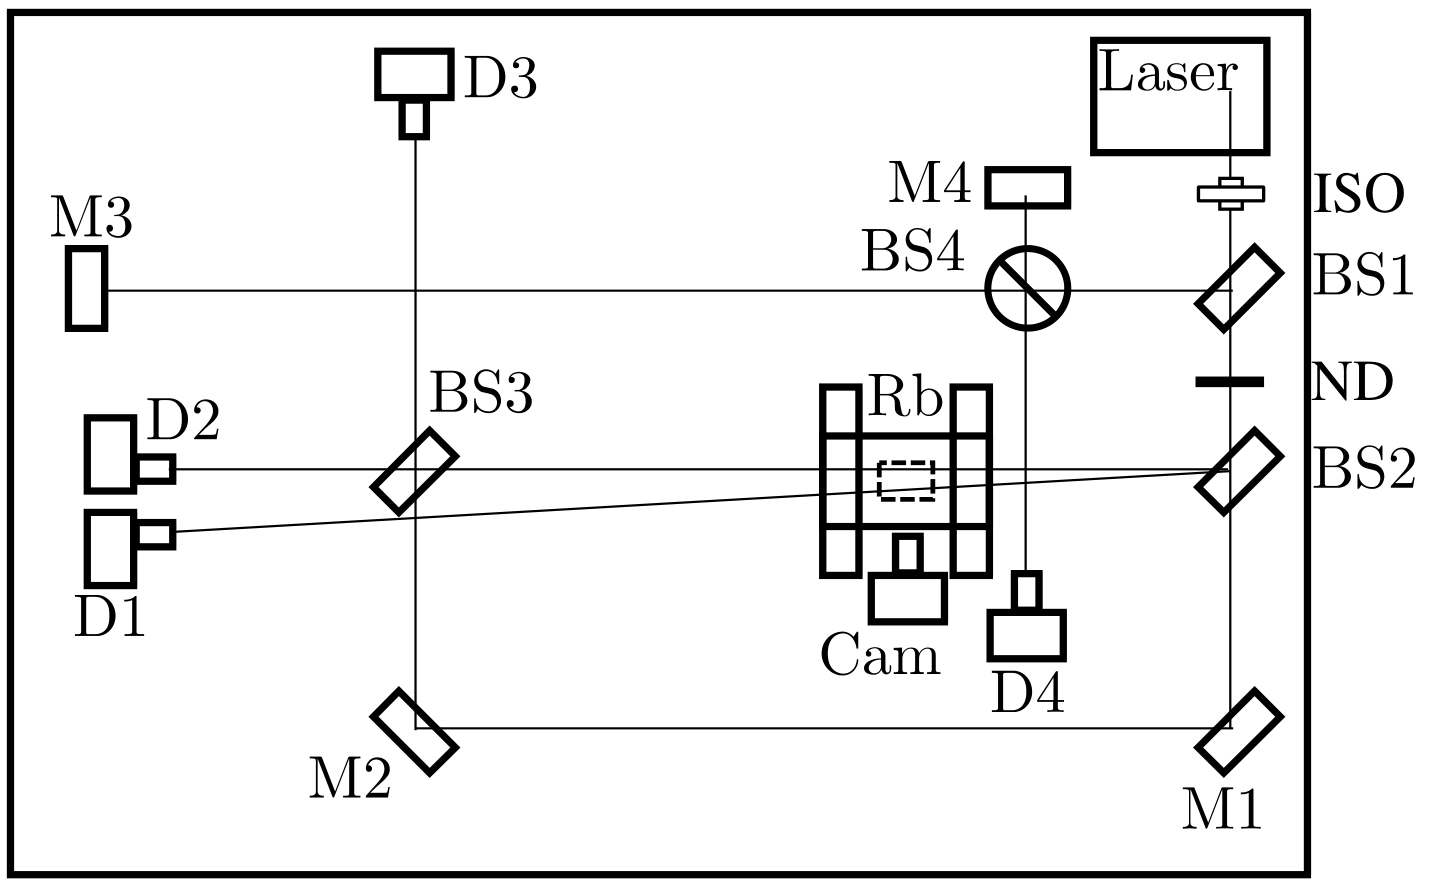
\includegraphics[ width = 0.8 \linewidth ]{apparatus.PNG}
    \caption{Schematic illustration of the apparatus}
    \label{fig:apparatus}
\end{figure}
The general setup that we used for all three experiments is shown in Figure \ref{fig:apparatus}. We make note that M1-M4 refer to mirrors, BS1-BS4 refer to beam splitters, D1-D4 refer to the detectors. Furthermore, ND refers to a filter (which is an almost black attenuator).

\subsection{The Controller}
\begin{figure}[H]
    \centering
    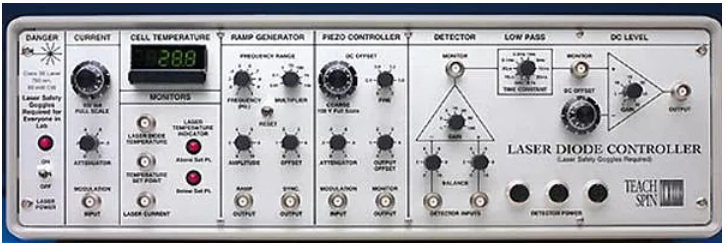
\includegraphics[ width = 0.8 \linewidth ]{controller.PNG}
    \caption{The controller for the TeachSpin diode laser}
    \label{fig:controller}
\end{figure}
The apparatus for this lab is controlled entirely the controller that is shown in Figure \ref{fig:controller}. The laser controls can be found at the far left, and we make sure that the dial that controls the current supplied to the laser is completely turned counter-clockwise before we turn on of off the laser. On top of being able to control the current supplied to the laser, we can control the temperature of the rubidium cell via the buttons that are connected with the LED display that tells us the current temperature within the cell. Beneath the temperature controller are laser status indicators that is of little concern to us.

The next key part of the controller would be the triangle wave "ramp generator". The dials at the top and middle control the frequency and amplitude of our triangle wave respectively. The outputs can be found at the bottom. 

To the right of the ramp generator would be the high voltage amplifier that powers the piezoelectric stack. An input signal and monitor output can be found at the bottom left and right respectively. The middle dials control the monitor output, and the DC offset controls can be found at the top. The piezo controller and ramp generator are used together to sweep the laser's wavelength. In particular, the absorption peak spectrum can be moved left or right on the oscilloscope by increasing or decreasing the DC offset. Furthermore, the spectrum can be spread out by reducing the amplitude of the generated ramp so that small details might be magnified.

Finally, the rightmost section contains a difference amplifier, a low-pass filter, and an amplifier with offset to allow processing signals for display and recording.

We note that we use an oscilloscope to display the output from the controller.

\subsection{The Laser}
\begin{figure}[H]
    \centering
    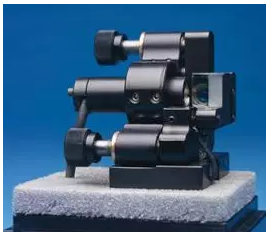
\includegraphics[ width = 0.8 \linewidth ]{laser.PNG}
    \caption{The TeachSpin diode laser}
    \label{fig:laser}
\end{figure}
The laser that we used in this lab was TeachSpin's diode laser as shown in Figure \ref{fig:laser}. This laser is special in that it is both temperature and current regulated; by varying the temperature, we are able to vary the diode laser's wavelength from about $770 - 795 \si{nm}$. Although the difference may seem small, we must note that this is a much more noticeable difference by the standard of atomic energy levels. 

\subsection{Absorption Cell Assembly}
As noted earlier, an absorption cell assembly consists of an outer glass cylinder, an insulation layer, a heater assembly, a "cold-finger" (which is a small piece of metal that fits over a small protusion on the side of the cell), a thermocouple to monitor the temperature, and the gas-filled rubidium cell. Furthermore, the assembly is mounted at the center of a pair of magnetic field coils.

\subsection{The Detectors}
The apparatus for this lab consisted of four PIN photodiode detectors labeled as D1-D4 (as shown in Figure \ref{fig:apparatus}). The key features of these detectors are that they contain current to voltage converters, and there is a dial at the back of each detector that allows us to change the gain setting from $10\si{M \Omega}$ to $333 \si{\Omega}$ in ten steps. These detectors also have separate signal and power cables, but we note that the controller can only handle three detectors at one time since there are only three power ports.

\subsection{TV and Camera}
The TV and camera allows for us to observe the light coming from the laser and the rubidium fluorescence in the vapor cell. 

\section{Measurements and Data Analysis}

\subsection{Data Collection}
\label{sec:data collection}
In this section, we will go more in depth on the experimental methods for each of the three experiments. 

\subsubsection{Observing the Absorption Spectrum for a Rubidium Vapor Cell}
For this part of the lab, we are only concerned about the output that we get from D2 in Figure \ref{fig:apparatus}. As noted in the apparatus section of this lab report, each of the detectors have separate signal and power cables. The power cable connects to one of the three available power ports in the controller, and the signal cable connects to one of the outputs of the ramp generator via a T-splitter. We are able to further connect the output of the ramp generator with the oscilloscope via the T-splitter as well.

With this, we are now able to to turn on the laser and make sure to gradually increase the current of the laser until we see the rubidium fluorescence in the vapor cell through the camera/TV. Once this is set up, we adjust several parameters so that the output displayed on the oscilloscope is well-scaled. For example, such parameters could be the gain on D2, the frequency and amplitude from the ramp generator, the current of the laser, etc.

The expected output that we should get is shown in Figure \ref{fig:resonant_peak_expected}. 

\begin{figure}[H]
    \centering
    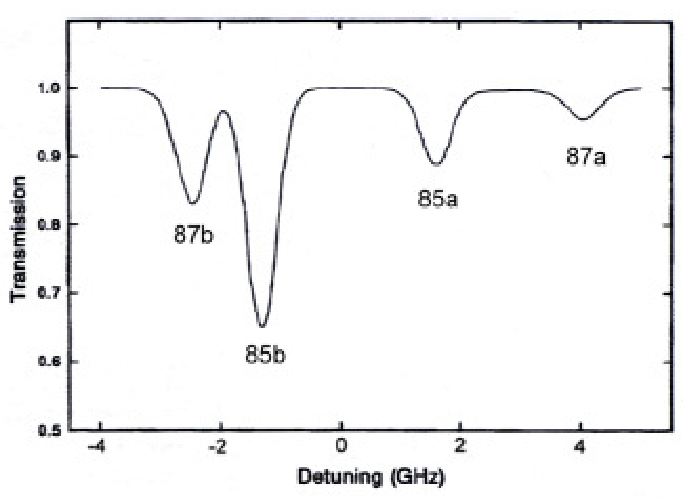
\includegraphics[ width = 0.8 \linewidth ]{resonant_peaks_expected.PNG}
    \caption{Typical absorption spectrum for a rubidium vapor cell.}
    \label{fig:resonant_peak_expected}
\end{figure}

The output that we ended up getting is shown in Figure \ref{fig:resonant_peaks}.

\begin{figure}[H]
    \centering
    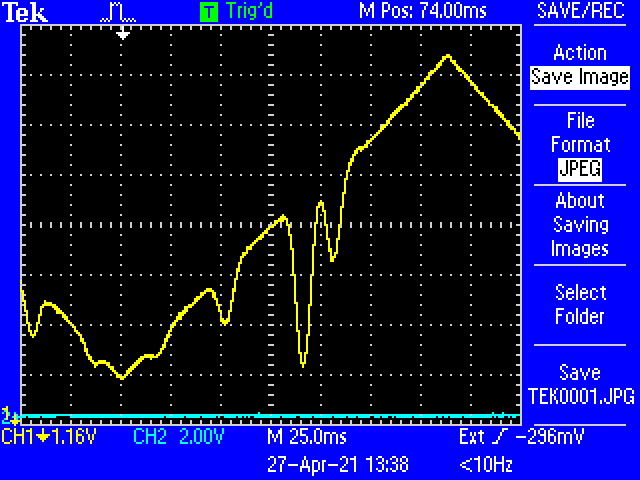
\includegraphics[ width = 0.8 \linewidth ]{resonant_peak.JPG}
    \caption{Measured absorption spectrum for a rubidium vapor cell.}
    \label{fig:resonant_peaks}
\end{figure}
Notice that the resonant peaks are superimposed on top of a triangle wave for our output due to the configurations we set for our ramp generator.

\subsubsection{Observing the p-state Hyperfine Splitting}
In this part of the lab, we now want to observe the hyperfine splitting of our rubidium vapor cell. As mentioned in the theory section, we are not able to just zoom in and look at the hyperfine structure due to Doppler broadening. Also mentioned in the theory section, we need to do perform a saturated absorption spectroscopy to unveil the hyperfine structure of our rubidium vapor cell. To set up this type of spectroscopy, we refer back to Figure \ref{fig:apparatus} and note that main components for such a setup includes BS1, BS2, D1, and D2. 

As we did with D1, we need to make sure that D2 is powered up. Note that we keep D1 set up as it was in the previous experiment but now connect D2 as an input for the difference amplifier. With this setup, the controller is able to unveil the fine details of the hyperfine splitting, and we are able to adjust several parameters again to make sure the the hyperfine structure is well-scaled. Again, we can adjust the gain on both the detectors as well as on the controller, adjust the amplitude, frequency, etc. to make sure that the hyperfine structure is zoomed in well. An example of one observed hyperfine structure is shown in Figure \ref{87b oscilloscope}. 

\subsubsection{Measuring the Hyperfine Splitting}
\label{sec:measure_hfs}
For the final experiment, we now want to measure the hyperfine splitting of our rubidium vapor cell. Most of the setup has already been done for us in the previous two experiments. The only thing that we need to include now is the interferometer. As shown in Figure \ref{fig:apparatus}, this consists of BS1, BS4, M3, M4, and D4. The importance of utilizing an interferometer is that it allows for us to calibrate the horizontal axis of the oscilloscope in units of frequency rather than time.

To make the calibration possible, we need to first calculate what the change in frequency of our laser is and then be able to connect this change in frequency with time. We start with the former and define the distance between M3 and BS4 to be $x_{1}$, and the distance between M4 and BS4 to be $x_{2}$. From this, we can see that after the laser splits into two beams, those two beams propagate their respective distances and are then recombined in the section between BS4 and D4. When the beams recombine, we have that there will be a phase difference caused by the difference in path length; this is given by 
\begin{equation}
    \Delta \phi 
    =
    2 \pi \frac{2 x_{1} - 2 x_{2}}{\lambda} 
    =
    \frac{4 \pi \Delta f}{c} ( x_{1} - x_{2} )
    \label{eq:measure_hfs-1}
\end{equation}
where we note that $\lambda$ is the wavelength of the laser and $\Delta f$ corresponds to the change in frequency. We note that because the laser is being swept by a triangle wave, changing the frequency will result in a phase difference as shown in equation \ref{eq:measure_hfs-1}. Barring the full details of the calculation (which can be found on page 13 of \cite{gatech}), we see that the frequency spacing between the interference maxima ends up being 
\begin{equation}
    \Delta f = \frac{c}{2 (x_{1} - x_{2})}
    \label{eq:measure_hfs-2}
\end{equation}
With this, we can now move onto how we might connect this with time on the oscilloscope. Notice that D4 can output the results from the interferometer. So, if we connect D4 to one of the available channels on the oscilloscope, we have that we can measure the period $T$ from maxima to maxima of our interference wave. Thus, we end up getting a conversion factor, since there is a certain $\Delta f$ across $T$. What this then allows for us to do is measure the hyperfine splitting of our rubidium vapor cell since we can read off the change in time from real peak to real peak and convert this change in time into frequency to get the change in frequency between the real peaks of the hyperfine splitting.

We finally note that we measure the change in frequency between the real hyperfine peaks since there are expected values that we can compare with (as shown in Figure \ref{fig:rubidium_splitting}). To make our notation clear, $85\mathrm{a}_{\mathrm{F}': 1, 2}$ refers to ${}^{85} \mathrm{Rb}$ where $F = 2$ with the difference in frequency pertaining to $F' = 1, 2$.

\subsection{Data Analysis}
\label{sec:data analysis}
In order to measure the hyperfine splitting for each of the four dips in the Rb absorption spectrum, we downloaded JPEG images of the oscilloscope display and corresponding CSV data files for each of the four dips, and read that data into a Python notebook to begin our analysis. We repeated the data collection and analysis several times for each Rb absorption dip, in order to ensure that our measurements were accurate and reported with an appropriate uncertainty. Figures \ref{87b oscilloscope} and \ref{fig:87b peaks} are examples of how our data looked for each measurement. We refrain from showing the others since the rest of the measurements looked similar to what is shown in Figures \ref{87b oscilloscope} and \ref{fig:87b peaks}. Furthermore, showing all the data would double the length of this lab report due to the amount of data that took for each peak.

\begin{figure}
    \centering
    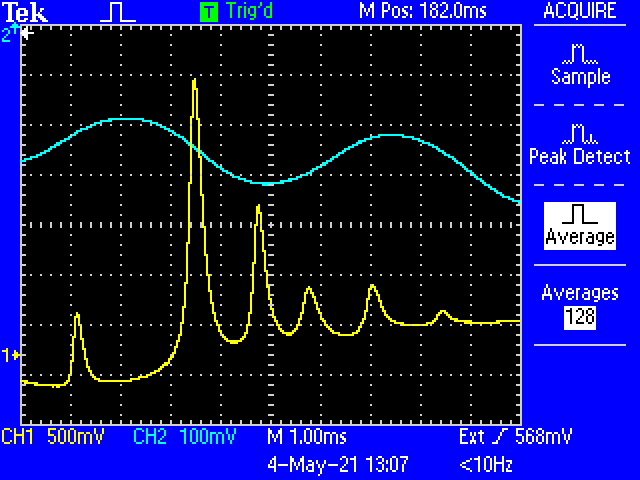
\includegraphics[width=0.425\textwidth]{figures/87b_1.JPG}
    \caption{An image of the oscilloscope display, showing the hyperfine peaks for the 87b absorption dip in the Rubidium spectrum.}
    \label{87b oscilloscope}
\end{figure}

We began our analysis of the oscilloscope data by identifying the location of the hyperfine splitting peaks for each of the absorption dips. In order to do so, we plotted the data we downloaded from the oscilloscope, and used the \texttt{scipy} find\_peaks function. Fig. \ref{fig:87b peaks} shows an example of this, where the orange line is our oscilloscope data, and the blue triangles are the peaks located in the data by \texttt{scipy} find\_peaks. In some cases, this process was aided by the use of the \texttt{scipy} savgol\_filter function, which was used to apply a Savitzky-Golay filter to smooth our data and make the peaks easier to identify. Further manual analysis was necessary to confirm that the peaks identified were accurate.

\begin{figure}
    \centering
    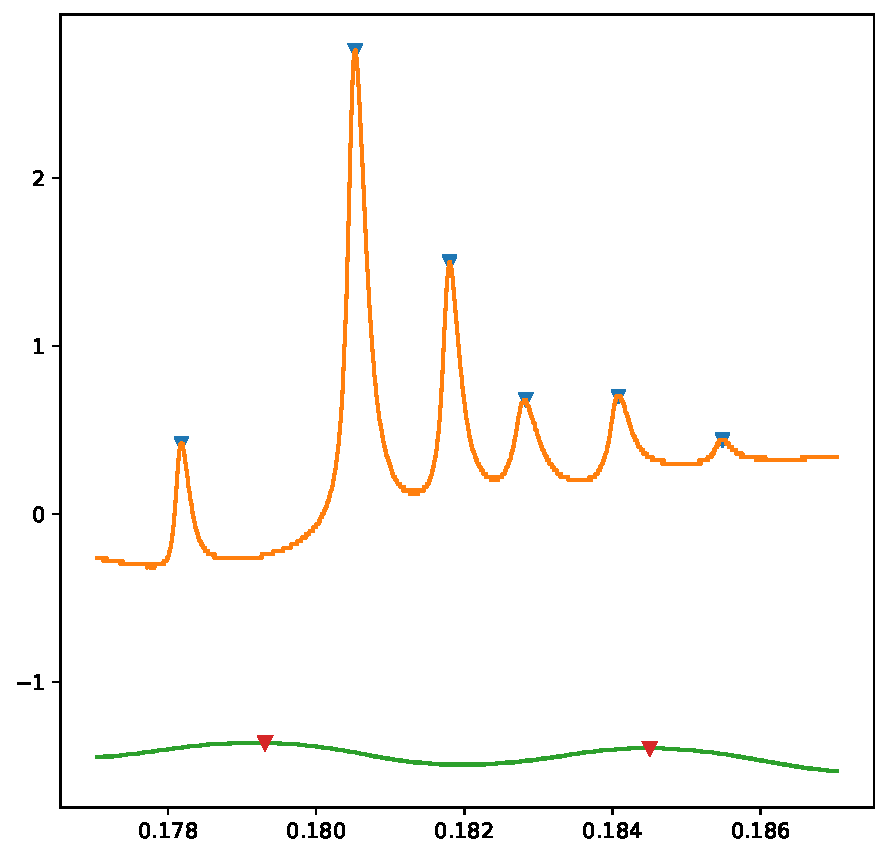
\includegraphics[width=0.425\textwidth]{figures/87b_1_peaks.pdf}
    \caption{An example of peak fitting, to identify the locations of the hyperfine peaks of the 87b absorption dip feature. Inflection points of the frequency displayed in CH2 of our oscilloscope were also identified (shown in red, on the green line), in order to determine the changes in freqency betweeen the hyperfine peaks by comparison.}
    \label{fig:87b peaks}
\end{figure}

In some cases, one or more of the peaks, though visible, was too shallow to be identified using these methods. In these cases, we fit a polynomial to a section of the data using the \texttt{numpy} function polyfit. We then subtracted off the polynomial from the data, in order to make the shallow peaks more prominent and easier to identify. In order to account for the shift in the peak that occurs when subtracting a fit, we identified the shift that occurred in some of the already well-identified peaks when the fit was subtracted, and applied that same shift to the peaks that were too shallow to identify prior to subtracting the fit. This process is shown in Figure \ref{fig:peak fitting}, and described in further detail in the caption of that figure. 

\begin{figure}
    \centering
    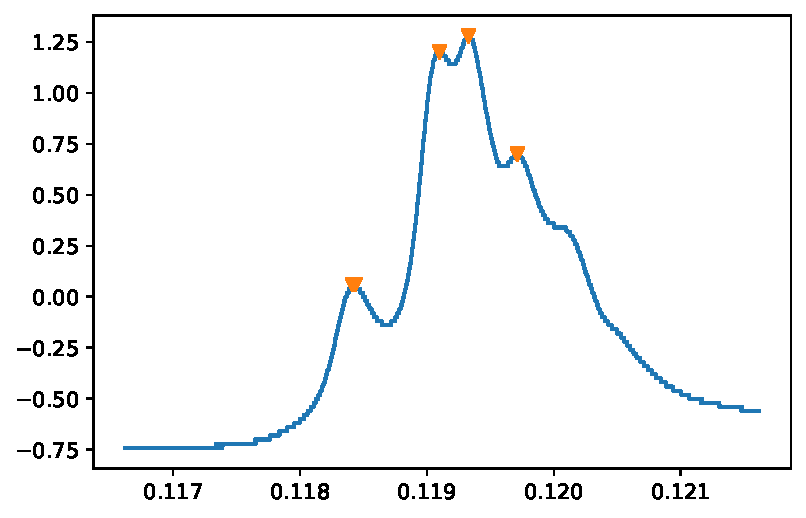
\includegraphics[width=0.22\textwidth]{figures/85a_missing.pdf}
    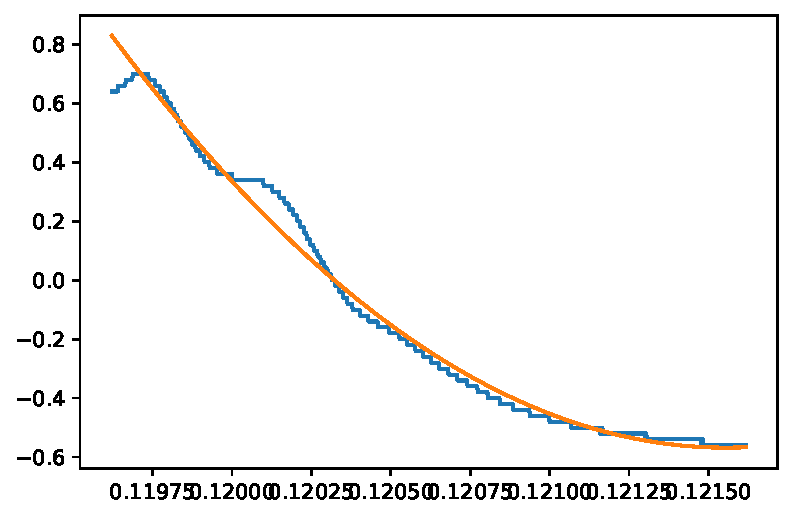
\includegraphics[width=0.22\textwidth]{figures/85a_polyfit.pdf}
    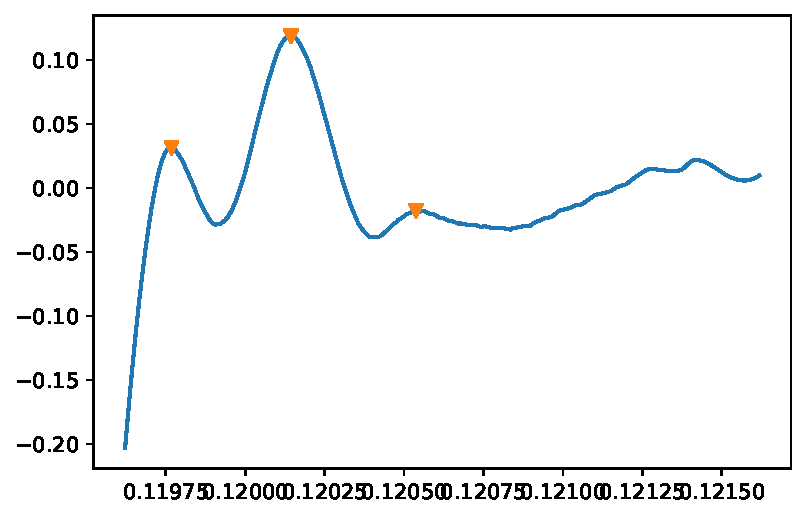
\includegraphics[width=0.22\textwidth]{figures/85a_polyfit_peaks.pdf}
    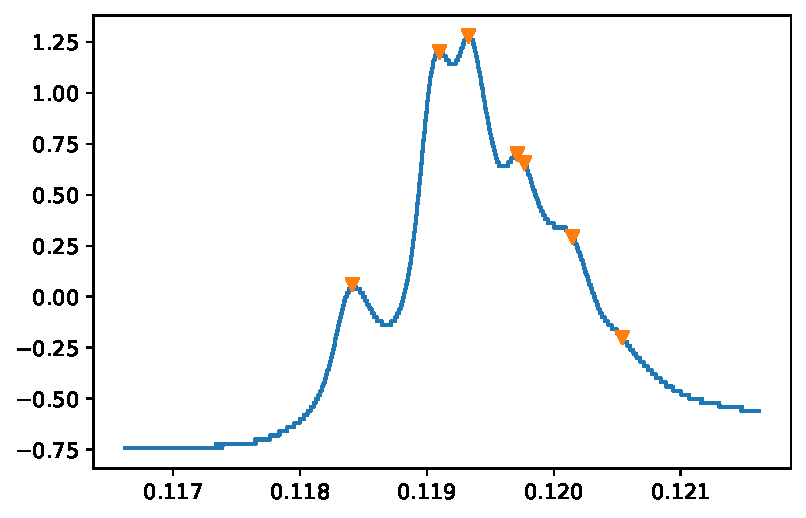
\includegraphics[width=0.22\textwidth]{figures/85a_allpeaks.pdf}
    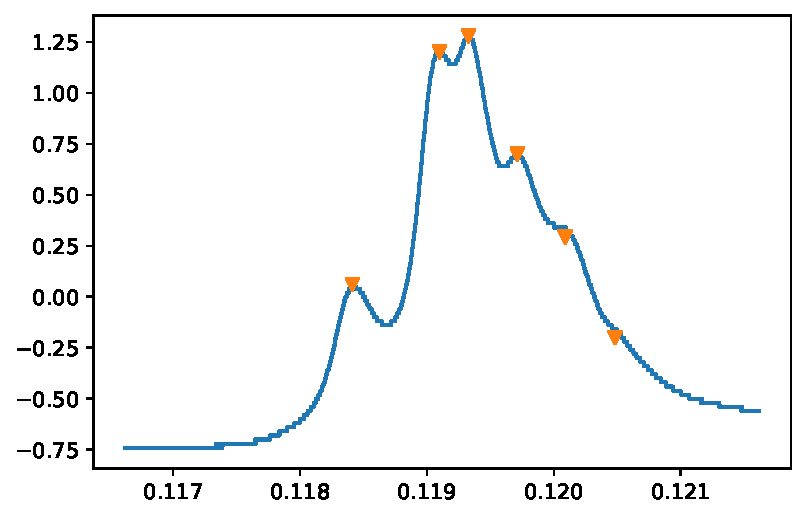
\includegraphics[width=0.22\textwidth]{figures/85a_finalpeaks.pdf}
    \caption{An example of peak fitting process when some of the peaks are too shallow to identify using the methods shown in Fig. \ref{fig:87b peaks}. The plot in the top left corner shows the initial results of attempting to locate the peaks of the hyperfine splitting structure of Rb 85a. In this case, the fifth and sixth peaks are too shallow to identify in this way. The top right plot shows a polynomial fit (shown in orange) to the last three peaks, and the middle left plot shows those peaks when the polynomial fit has been subtracted off. In this case, each peak is now clearly identifiable. The middle right plot shows the combination of the peaks identified in the first (top left) plot, and the peaks identified in the third (middle left) plot. As you can see, the fourth peak has two orange triangles indicating the peak location; one from the first plot and one from the second. In finding the difference between these two results for the fourth peak, we can then know by how much the polynomial subtraction has shifted the location of the peaks, and apply a correction to the fifth and sixth peaks. The final plot on the bottom shows the result; each of the six peaks has been located, and the correction has been applied to the fifth and sixth peaks, moving them slightly to the left of their position in the fourth (middle right) plot.}
    \label{fig:peak fitting}
\end{figure}

Once accurate peaks were identified, it was then necessary to identify which peaks corresponded to real hyperfine splitting features, and which were crossover resonances as discussed in Section \ref{sec:crossover resonances}. Knowing that the peaks on each end (far left and far right) could not be crossover resonances, we calculated the mean of those peak locations, and located the peak at that mean location, noting it to be a crossover resonance. Through similar calculations with the other peaks, we identified which of the middle peaks was a real artifact of hyperfine splitting. We created an array of the locations of the real peaks for use in our calculations.

Once we had identified the locations of the real peaks, we made use of the same smoothing and peak fitting methods to find inflection points of the interferometer signal displayed in CH2 of our oscilloscope (confer Figure \ref{87b oscilloscope}).
With the inflection points known, we are able to calculate the period, $T$, between two maximas.

As noted in Section \ref{sec:measure_hfs}, the interferometer signal came from detector D4, and we use this signal in order to calibrate the horizontal axis in units of frequency rather than time. The calibration requires that we know the period, $T$, between two maximas (which we already found above) and the frequency spacing, say $\Delta f$, between those two two maximas as well. We can calculate $\Delta f$ by utilizing equation \ref{eq:measure_hfs-2}. Our measured values for $x_{1}$ and $x_{2}$ ended up being the following:
\begin{equation}
    x_{1} = 53.6 \pm 0.1 \si{cm}
    \quad \mathrm{and} \quad 
    x_{2} = 5.2 \pm 0.1 \si{cm}
    \label{eq:da-1}
\end{equation} 
With this, we have that 
\begin{equation}
    \Delta x
    =
    x_{1} - x_{2}
    =
    48.4 \pm \sigma_{\Delta x} \si{cm}
    \label{eq:da-2}
\end{equation}
where
\begin{equation}
    \sigma_{\Delta x}
    =
    \sqrt{ 0.1^{2} + 0.1^{2} }
    =
    0.14
    \label{eq:da-3}
\end{equation} 
Thus, we have via equation \ref{eq:measure_hfs-2}
\begin{equation}
    \Delta f
    =
    \frac{c}{2 \Delta x}
    =
    3.1 \times 10^{8} \si{Hz} \pm \left\lvert \sigma_{\Delta f} \right\rvert
    \label{eq:da-4}
\end{equation}
where
\begin{equation}
    \left\lvert \sigma_{\Delta f} \right\rvert
    =
    \Delta f \frac{\sigma_{\Delta x}}{\Delta x}
    =
    \frac{c}{2} \frac{\sigma_{\Delta x}}{(\Delta x)^{2}}
    =
    6.4 \times 10^{3} \si{Hz}
    \label{eq:da-5}
\end{equation}
With $\Delta f$ and $T$ calculated and known, we could then calculate the change in frequency $\Delta f_{peaks}$ between our hyperfine peaks, by calculating: 
\begin{equation}
    \Delta f_{peaks} = \frac{\Delta t \Delta f}{T} \pm \sigma_{\Delta f_{peaks}}
    \label{eq:da-6}
\end{equation}
where 
\begin{equation}
    \sigma_{\Delta f_{peaks}}
    =
    \Delta f_{peaks} \frac{\sigma_{\Delta f}}{\Delta f} + \sigma_{meas.}
    =
    \frac{\Delta t}{T} \sigma_{\Delta f} + \sigma_{meas.}
    \label{eq:da-7}
\end{equation}
where $\Delta t$ is the distance in time between each consecutive, real hyperfine splitting peak, and $\sigma_{meas.}$ is the standard deviation of multiple trials of measuring $\Delta f_{peaks}$.

\subsection{Results}
The results of our measurements are shown in Table \ref{tab:results}. The Hyperfine Transition column refers to the hyperfine splitting as discussed in Section \ref{sec:structure} and shown in more detail in Fig. \ref{fig:rubidium_splitting}. 
\begin{table}[H]
\centering
\caption{Hyperfine Splitting Results} 
\label{tab:results}
% \renewcommand{\arraystretch}{1.3}
\begin{tabular}{||l|c|c||}
 \hline
 \bf Hyperfine & $\Delta f_{peaks}$ & Expected $\Delta f_{peaks}$\\
    \bf Transition &  (GHz) & (GHz) \\
 \hline
 \bf $85\mathrm{a}_{\mathrm{F}': 1, 2}$ & $0.0306 \pm 0.0027$ & $0.029$ \\
 \bf $85\mathrm{a}_{\mathrm{F}': 2, 3}$ & $0.0555 \pm 0.0029$ & $0.063$ \\
 \bf $85\mathrm{b}_{\mathrm{F}': 2, 3}$ & $0.0658 \pm 0.0009$ & $0.063$ \\
 \bf $85\mathrm{b}_{\mathrm{F}': 3, 4}$ & $0.1203 \pm 0.0033$ & $0.121$ \\
 \bf $87\mathrm{a}_{\mathrm{F}': 0, 1}$ & $0.0725 \pm 0.0020$ & $0.072$ \\
 \bf $87\mathrm{a}_{\mathrm{F}': 1, 2}$ & $0.1549 \pm 0.0023$ & $0.157$ \\
 \bf $87\mathrm{b}_{\mathrm{F}': 1, 2}$ & $0.1562 \pm 0.0024$ & $0.157$ \\
 \bf $87\mathrm{b}_{\mathrm{F}': 2, 3}$ & $0.2695 \pm 0.0055$ & $0.287$ \\
 \hline
\end{tabular}
\end{table}

% \begin{tabular}{ |p{3cm}||p{3cm}|  }
%  \hline
%  \multicolumn{2}{|c|}{Hyperfine Splitting Results} \\
%  \hline
%  \bf{Hyperfine Transition} & $\Delta f_{peaks}$\\
%  \hline
%  \bf 85a_{2 to 1}     & $0.0324 \pm 0.0007$\\
%  \bf 85a_{2 to 3}     & $0.0555 \pm 0.0027$\\
% %  Albania &AL & ALB&  008\\
% %  Algeria    &DZ & DZA&  012\\
% %  American Samoa&   AS  & ASM&016\\
% %  Andorra& AD  & AND   &020\\
% %  Angola& AO  & AGO&024\\
%  \hline
% \end{tabular}

The second column of Table \ref{tab:results} ($\Delta f_{peaks}$), shows our results, obtained through the measurements and analysis described in Sections \ref{sec:data collection} and \ref{sec:data analysis}. Each result is the mean result obtained through several trials. The uncertainties cited in the table are the sum of the standard deviation of the measurements, and the propagated uncertainty from the measurement of $\Delta x$, as discussed in Section \ref{sec:data analysis}. The third column of the table (Expected $\Delta f_{peaks}$) shows the expected values from theory. These are also found in Figure \ref{fig:rubidium_splitting}.   

\section{Discussion}
\label{sec:discussion}
% Discuss the extent to which your results are consistent with what you would theoretically predict, and explain why you think that you have the observed level of agreement/disagreement.  What experimental factors limited the precision, accuracy, and scope of your measurements?
With a few exceptions, our results are generally consistent with what we expect from theory. All but three of our results are within $1 \sigma$ of the expected result. The exceptions are: $85\mathrm{a}_{\mathrm{F}': 2, 3}$, which is within $3 \sigma$; $85\mathrm{b}_{\mathrm{F}': 2, 3}$, which is within $4 \sigma$, and $87\mathrm{b}_{\mathrm{F}': 2, 3}$, which is within $4 \sigma$. 

The agreement between our results in general is encouraging, and leads us to believe that our apparatus was basically well-tuned. However, certain data collection and analysis methods limited the accuracy of our measurements. 

One possible source of error which is not currently reflected in our uncertainties is the uncertainty in locating our peaks. This process was done using a python script designed to locate the peaks to a greater precision than could have been achieved by eye, but uncertainties still exist in this measurement. The peaks which were located by first subtracting a polynomial fit, as described in Fig. \ref{fig:peak fitting}, are the most uncertain; the peaks were shallow to start, and then a shift was introduced by flattening the curve. Though we did attempt to correct for this shift, the fit is a second order polynomial, so the exact shift that subtracting the fit introduces will be slightly different at each point along the fit. Even the peaks which were located without subtracting a fit are somewhat uncertain: we employed a Savitzky-Golay smoothing filter to some of the hyperfine peaks if the curve from the oscilloscope was choppy, and this could have introduced uncertainty by shifting the peaks slightly from their original position in the process of smoothing the curve. 

Another possible source of error that we need to consider would be the systematic error of our apparatus. As discussed with Prof. Watkins, the oscilloscope is only specific within 1\%, and the diode laser controller adds an uncertainty of around 2-3\% for our output. Furthermore, we note that the apparatus is highly sensitive to vibrations, so any outside interference from the movements of the table or apparatus would have resulted in our measurements to vary wildly. For example, just putting an arm on the lid of the apparatus produced noticeable fluctuations in the output when looking at the oscilloscope. With this, our measurements could have an uncertainty greater than what we have shown in Table \ref{tab:results} as a result. 

In addition to the apparatus being highly sensitive to vibrations, we note that the alignment of the laser, mirrors, beam-splitters, and detectors were also very sensitive to change. Having one mirror being misaligned could result in the interferometer to send over incorrect information, and it could also result in our saturated absorption spectroscopy to not be saturated enough if the alignment is off enough. This could have been the case in our scenario since several of our measurement were not able to unveil the sixth hyperfine peak. Thus, this could result in the values that we did get for the five other hyperfine peaks to vary from what they were supposed to be. 

Another potential reason for why we could not unveil the sixth hyperfine peak could be that our laser is showing its age. As Prof. Watkins mentioned during our lab, the laser could have been worn down over the years. This results in the uncertainty of the laser to increase, and it could have also prevented us from seeing the sixth hyperfine peak. 

\section{Conclusion}

% Summarize the results of your experiment, and comment on how could the experiment could potentially be improved in the future.
In this lab we were generally successful in measuring the hyperfine splitting of a rubidium vapor cell. Our results, summarized in Table 1, are mostly within $1 \sigma$ of the expected values. The exceptions to this are $85\mathrm{a}_{\mathrm{F}': 2, 3}$, $85\mathrm{b}_{\mathrm{F}': 2, 3}$, and $87\mathrm{b}_{\mathrm{F}': 2, 3}$, which are each within $4 \sigma$ at most. 

Various sources of potential error that are not currently reflected in our uncertainties are discussed in Section \ref{sec:discussion}. In order to obtain better results, we suggest that future attempts at this lab make efforts to mitigate those sources of error.

One possible improvement would be to better account for error in the peak fitting process. Acknowledging uncertainty in the exact location of the peaks would be especially useful for the peaks with the most uncertain locations: the ones for which a polynomial fit had to be subtracted to locate the peak. In this lab, we cropped a section of the data closely surrounding these shallow peaks, including only one or two non-shallow peaks, and fit a polynomial to just that section. In the future, a polynomial could be fit and subtracted from the entire range of data, including all of the peaks, and a shift correction could be calculated from each of the already-located peaks. This would give several shift values, and provide an uncertainty on the shift correction, which is certainly not accurate to the precision that we assumed in this lab. 

Another improvement to this lab would be better isolating the apparatus. Within the limitations of our lab environment, this would be difficult to do, but in order to obtain more precise measurements it would be better to conduct measurements in an isolated room where there is minimal noise and movement causing possibly disruptive vibrations. 


\section{Figure References}
Figure \ref{fig:rubidium_splitting}, \ref{fig:apparatus}, and \ref{fig:resonant_peak_expected} can be found in the lab manual under the section for rubidium spectroscopy. Figures \ref{fig:controller} and \ref{fig:laser} can be found on \cite{teachspin}.

\bibliographystyle{unsrt}
\bibliography{References}

\end{document}